\documentclass[dvipsnames, 10pt]{beamer}
\beamertemplatenavigationsymbolsempty
\setbeamertemplate{footline}[frame number]
\usecolortheme[named=RoyalBlue]{structure}
\usefonttheme{serif}
\usepackage{amsmath, amssymb}
\usepackage{multirow, booktabs, tabularx, colortbl, xcolor}
\usepackage{caption, subcaption}
\usepackage{tikz}
\usetikzlibrary{arrows.meta, positioning}
\graphicspath{{figures/}}

\AtBeginSection{\frame{\sectionpage}}

\definecolor{adultc}{HTML}{33475B}
\definecolor{childc}{HTML}{2A9D8F}

\author{Hyunwoo Cho}
\institute{National Institute for Mathematical Sciences}
\date{August 4, 2026}
\title{An age-structured contact model of sick-leave and school-absence effects on seasonal influenza in Korea}

\begin{document}

\maketitle

\begin{frame}\frametitle{Contents}
    \tableofcontents[subsectionstyle=hide]
\end{frame}

%%%%%%%%%%%%%%%%%%%%%%%%%%%%%%%%%%%%%%%%%%%%%%%%%%%%%%%%%%%%%%%%%
\section{Background}

\begin{frame}\frametitle{Two absenteeism levers, unequal evidence}
    \begin{itemize}
        \item Keeping infectious individuals out of a shared setting is a standard
              non-pharmaceutical response to influenza:
              \begin{itemize}
                  \item \textbf{school exclusion} for symptomatic children;
                  \item \textbf{sick leave} for symptomatic workers.
              \end{itemize}
        \item Keeping children out of school is comparatively well-studied.
              Keeping adults home from work is \textbf{far less established}.
        \item The intuitive case for both is the same: an infectious person who
              stays home cannot infect the colleagues or classmates they would
              have met --- so evaluations have concentrated on the \textbf{size of
              that reduction}.
        \item The two levers have rarely been compared on the \textbf{same
              footing}, in one model and for the same seasons.
    \end{itemize}
\end{frame}

\begin{frame}\frametitle{What a single ``effect size'' omits}
    For an age-structured respiratory pathogen, an aggregate effect size hides
    four things:
    \begin{itemize}
        \item \textbf{Heterogeneity.} Susceptibility, attack rate, and contacts
              vary sharply by age; children are among the most susceptible and,
              in most seasons, the most infectious group.
        \item \textbf{Redistribution.} Sending an infectious person home does not
              end their transmission --- it \textbf{relocates} it into the
              household, whose age mix differs from the setting they left.
        \item \textbf{Presymptomatic transmission.} A share of influenza~A spreads
              before symptoms, beyond the reach of any symptom-triggered policy.
        \item \textbf{Timing.} The household is always open, even when schools are
              not, so a policy that shifts transmission home behaves differently
              in term than in the winter break.
    \end{itemize}
\end{frame}

\begin{frame}\frametitle{Aims}
    We built an age-structured SVEIR model of seasonal influenza in the Seoul
    Capital Area to move from ``how much is averted'' to ``\textbf{whom} does the
    policy move risk toward, \textbf{with what certainty}, and \textbf{when}.''
    The model lets us:
    \begin{itemize}
        \item[(i)] compare sick-leave and school-absence policies at matched
              intensity, on the same footing, with credible intervals;
        \item[(ii)] locate where in the workplace-transmission / crowding
              parameter space sick leave helps versus harms;
        \item[(iii)] decompose outcomes by age and by metric (rate vs.\ count);
        \item[(iv)] ask how the same sick-leave policy behaves in different phases
              of the epidemic, split by the winter-break calendar.
    \end{itemize}
\end{frame}

%%%%%%%%%%%%%%%%%%%%%%%%%%%%%%%%%%%%%%%%%%%%%%%%%%%%%%%%%%%%%%%%%
\section{Model assumptions}

\begin{frame}\frametitle{Household spillover: the mechanism}
    \centering
    \resizebox{0.98\textwidth}{!}{%
    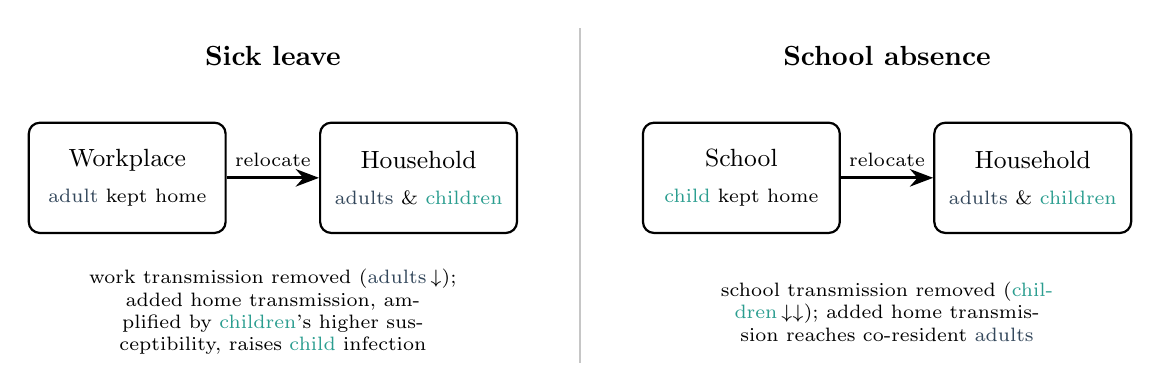
\begin{tikzpicture}[>=Stealth, font=\small,
      place/.style={draw, thick, rounded corners, minimum width=25mm, minimum height=14mm, align=center, inner sep=3pt},
      arr/.style={->, very thick},
      net/.style={font=\scriptsize, align=center, text width=52mm}]
    \node[font=\bfseries] at (0.15,1.55) {Sick leave};
    \node[place] (wA) at (-1.7,0) {Workplace\\[2pt]{\scriptsize\textcolor{adultc}{adult} kept home}};
    \node[place] (hA) at (2.0,0) {Household\\[2pt]{\scriptsize\textcolor{adultc}{adults} \& \textcolor{childc}{children}}};
    \draw[arr] (wA) -- node[above,font=\scriptsize]{relocate} (hA);
    \node[net] at (0.15,-1.7) {work transmission removed (\textcolor{adultc}{adults}\,$\downarrow$); added home transmission, amplified by \textcolor{childc}{children}'s higher susceptibility, raises \textcolor{childc}{child} infection};
    \draw[gray!45, thin] (4.05,1.9) -- (4.05,-2.35);
    \node[font=\bfseries] at (7.95,1.55) {School absence};
    \node[place] (sB) at (6.1,0) {School\\[2pt]{\scriptsize\textcolor{childc}{child} kept home}};
    \node[place] (hB) at (9.8,0) {Household\\[2pt]{\scriptsize\textcolor{adultc}{adults} \& \textcolor{childc}{children}}};
    \draw[arr] (sB) -- node[above,font=\scriptsize]{relocate} (hB);
    \node[net] at (7.95,-1.7) {school transmission removed (\textcolor{childc}{children}\,$\downarrow\downarrow$); added home transmission reaches co-resident \textcolor{adultc}{adults}};
    \end{tikzpicture}}
    \vspace{0.2cm}
    \begin{itemize}\small
        \item Home contacts: a child's are $\approx$80\% with adults; an adult's
              are $\approx$78\% with other adults.
        \item The net direction differs because the removed source and the
              household age mix differ.
    \end{itemize}
\end{frame}

\begin{frame}\frametitle{Household spillover: formulation}
    Baseline attendance is a retention fraction $p$ (kept attending while
    symptomatic); the policy lowers $p$, sending a fraction $1-p$ home. Only the
    symptomatic block $I_{23}$ is affected; the home-channel symptomatic
    prevalence is scaled by
    \begin{equation*}
        1 + \kappa_b\,(1-p)_b ,
        \qquad
        (1-p)_b =
        \begin{cases}
            1 - p_{\mathrm{school}}, & \text{students},\\
            \rho_b\,(1 - p_{\mathrm{work}}), & \text{workers},\\
            0, & 70+,
        \end{cases}
    \end{equation*}
    \begin{itemize}\small
        \item $\kappa_b$ = per-group increase in effective household transmission
              from a symptomatic person staying home; $\rho_b$ = employment rate
              (students $\rho_b=0$, no commute).
        \item $\kappa$ is \textbf{derived, not fitted} --- from the 2024 Korean
              Time-Use Survey (increase in home-stay time on a non-attendance vs.\
              attendance day). Spillover is an input, so the result is not circular.
    \end{itemize}
\end{frame}

\begin{frame}\frametitle{Presymptomatic transmission}
    \begin{itemize}
        \item The Erlang(3) infectious period $I_1\!\to\!I_2\!\to\!I_3$ gives a
              distinct \textbf{presymptomatic} sub-stage $I_1$: infectious but not
              yet symptomatic.
        \item Symptoms --- and any symptom-triggered behaviour (care-seeking,
              absenteeism) --- begin at $I_1\!\to\!I_2$. Both policies act only on
              $I_2, I_3$; the observation model (NHIS) is placed at symptom onset.
        \item $I_1$ transmits at reduced weight $w=0.22$
              ($\Rightarrow$ presymptomatic share $w/(w+2)\approx 9.9\%$),
              following a recent influenza~A household study.
        \item \textbf{Consequence:} presymptomatic transmission sets a
              \textbf{ceiling} on what any symptom-based policy can achieve ---
              much of a sick worker's transmission has already occurred, or occurs
              through $I_1$ contacts the policy never reaches.
    \end{itemize}
\end{frame}

\begin{frame}\frametitle{The school calendar acts on contacts, not on \texorpdfstring{$\beta$}{beta}}
    \begin{columns}[T]
        \column{0.52\textwidth}
        \begin{itemize}\small
            \item Each channel's matrix is a trapezoidal-in-time blend of a
                  school-term and a winter-break matrix:
            \[
                C^{c}_{ab}(t) = (1-h(t))\,C^{c,\mathrm{term}}_{ab}
                              + h(t)\,C^{c,\mathrm{vac}}_{ab},
            \]
            with $h(t)$ the winter-break ramp.
            \item Matrices are from a nationwide Korean (NIMS) contact survey,
                  term and break measured separately.
            \item Putting the calendar in $C(t)$ (not $\beta_{\mathrm{school}}$)
                  keeps the baseline home spillover $\equiv 1.0$ across the year ---
                  contact frequency and intervention intensity never contaminate
                  each other.
        \end{itemize}
        \column{0.48\textwidth}
        \centering
        
\includegraphics[width=\textwidth]{contact_matrices}\\
        {\scriptsize Contact matrices by channel, school term vs.\ winter break.}
    \end{columns}
\end{frame}

\begin{frame}\frametitle{Susceptibility, seasonal forcing, vaccination}
    \begin{itemize}
        \item \textbf{Age susceptibility $\phi_a$:} linear U-shape --- child anchor
              $2.0$ (0--4), working-age floor $1.0$ (20--44), elderly $1.5$ (70+),
              intermediate bands interpolated.
        \item \textbf{Seasonal forcing:}
              $s_f(t)=1+0.9\cos\!\big(\tfrac{2\pi(t-105)}{365}\big)$, peaking in
              mid-December.
        \item \textbf{Vaccination:} time-distributed leaky-protection hazard
              $v(t)=\tfrac{-\ln(1-C)}{Z}\,\mathrm{density}(t)$, normalized to reach
              target coverage $C=0.30$; efficacy $\mathrm{VE}=0.5$.
    \end{itemize}
\end{frame}

%%%%%%%%%%%%%%%%%%%%%%%%%%%%%%%%%%%%%%%%%%%%%%%%%%%%%%%%%%%%%%%%%
\section{Model and methods}

\begin{frame}\frametitle{Age-structured SVEIR compartmental structure}
    \begin{columns}[T]
        \column{0.5\textwidth}
        {\small For each of 15 five-year age groups $a$:}
        \begin{align*}
            \tfrac{dS_a}{dt}   &= -\lambda_a S_a - v(t)S_a,\\
            \tfrac{dV_a}{dt}   &= v(t)S_a - (1{-}\mathrm{VE})\lambda_a V_a,\\
            \tfrac{dE_a}{dt}   &= \lambda_a S_a + (1{-}\mathrm{VE})\lambda_a V_a - \sigma E_a,\\
            \tfrac{dI_{1,a}}{dt}&= \sigma E_a - 3\gamma I_{1,a},\\
            \tfrac{dI_{2,a}}{dt}&= 3\gamma I_{1,a} - 3\gamma I_{2,a},\\
            \tfrac{dI_{3,a}}{dt}&= 3\gamma I_{2,a} - 3\gamma I_{3,a},\\
            \tfrac{dR_a}{dt}   &= 3\gamma I_{3,a}.
        \end{align*}
        \column{0.5\textwidth}
        \centering
        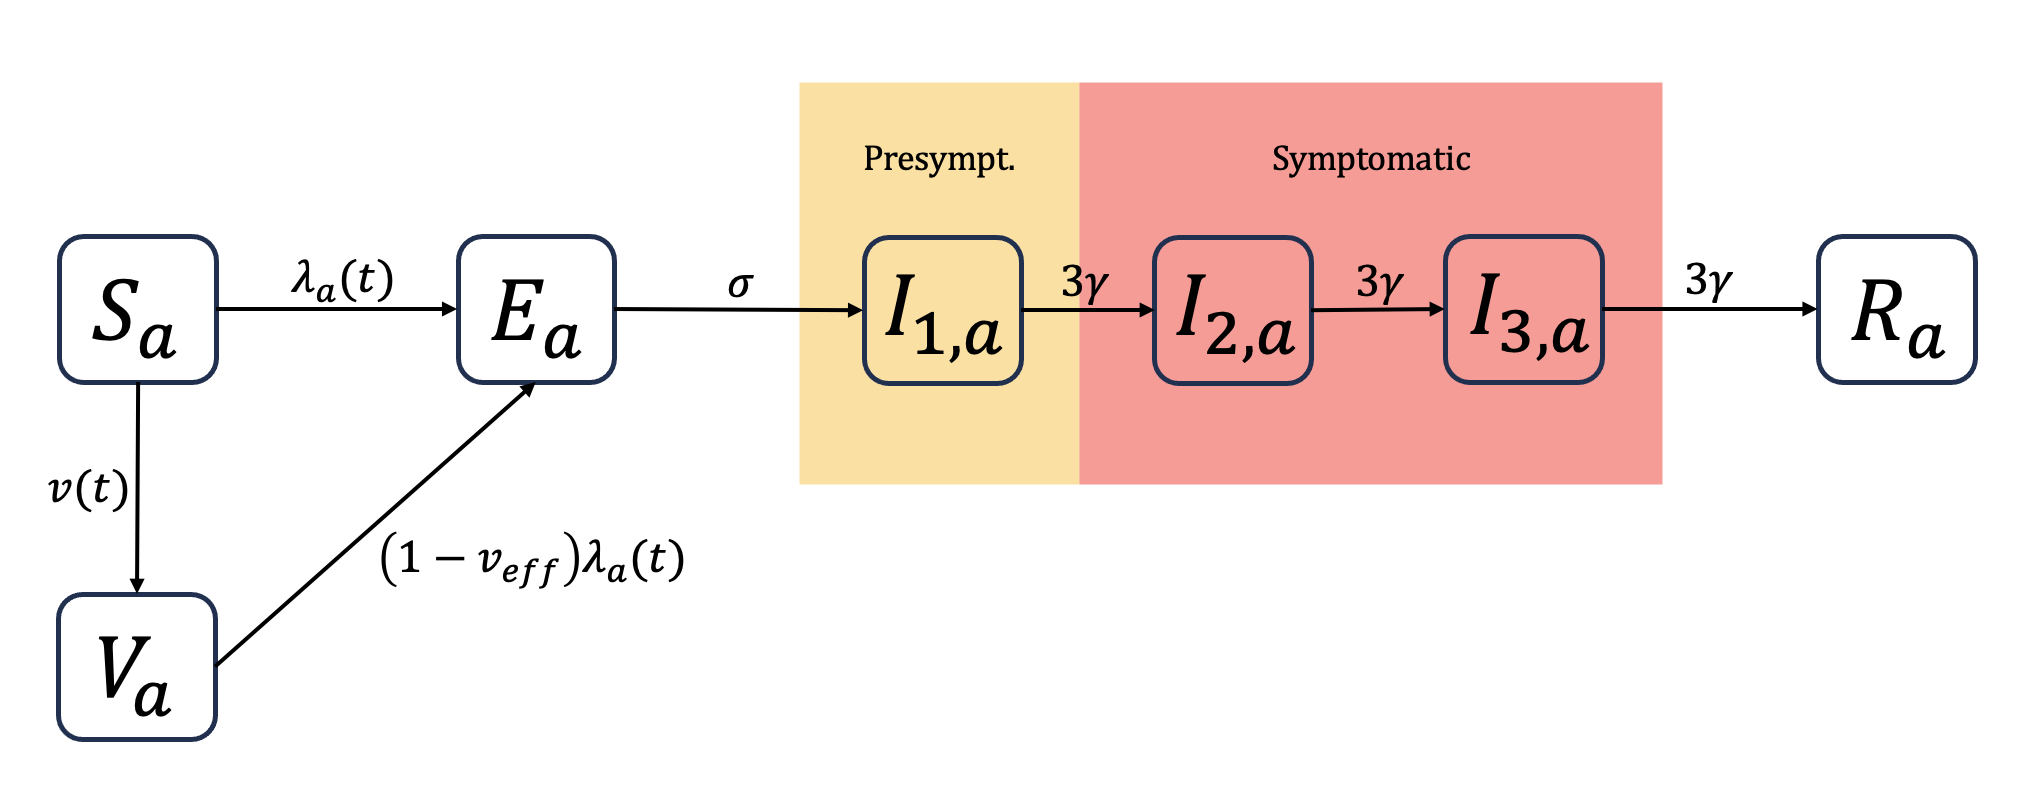
\includegraphics[width=\textwidth]{flow_diagram}\\
        {\scriptsize Latent period $1/\sigma=2$ d; mean infectious period
        $1/\gamma=4$ d over an Erlang(3) chain. $I_1$ presymptomatic (weight $w$),
        $I_2,I_3$ symptomatic (policy acts here).}
    \end{columns}
\end{frame}

\begin{frame}\frametitle{Force of infection: four contact channels}
    {\small With $I_{23,b}=I_{2,b}+I_{3,b}$, the channel hazards are}
    \begin{align*}
        \lambda^{\mathrm{work}}_a   &= \phi_a s_f(t)\,\beta_{\mathrm{work}} \textstyle\sum_b C^{\mathrm{work}}_{ab}(t)\,\frac{w I_{1,b} + p_{\mathrm{work}} I_{23,b}}{N_b},\\
        \lambda^{\mathrm{school}}_a &= \phi_a s_f(t)\,\beta_{\mathrm{school}} \textstyle\sum_b C^{\mathrm{school}}_{ab}(t)\,\frac{w I_{1,b} + p_{\mathrm{school}} I_{23,b}}{N_b},\\
        \lambda^{\mathrm{home}}_a   &= \phi_a s_f(t)\,\beta_{\mathrm{home}} \textstyle\sum_b C^{\mathrm{home}}_{ab}(t)\,\frac{w I_{1,b} + (1+\kappa_b(1-p)_b) I_{23,b}}{N_b},\\
        \lambda^{\mathrm{other}}_a  &= \phi_a s_f(t)\,\beta_{\mathrm{other}} \textstyle\sum_b C^{\mathrm{other}}_{ab}(t)\,\frac{w I_{1,b} + I_{23,b}}{N_b},
    \end{align*}
    {\small with $\lambda_a=\sum_c\lambda^c_a$. The presymptomatic block $wI_1$
    passes through every channel unaffected; policy retention
    $p_{\mathrm{work}},p_{\mathrm{school}}$ and the home crowding term act only on
    $I_{23}$.}
\end{frame}

\begin{frame}\frametitle{Transmissibility allocation and \texorpdfstring{$R_0$}{R0}}
    \begin{itemize}
        \item Scale and allocation are separated:
        \[
            \beta_c = \frac{R_0}{\rho_{\mathrm{eff}}(\pi,\phi)}\,\pi_c,
            \qquad \textstyle\sum_c \pi_c = 1,
        \]
        with $R_0$ setting the size and $\pi=(\pi_{\mathrm{home}},
        \pi_{\mathrm{work}},\pi_{\mathrm{school}},\pi_{\mathrm{other}})$ the allocation.
        \item $\rho_{\mathrm{eff}}$ is the dominant next-generation eigenvalue,
              adjusted for presymptomatic infectiousness:
              $\rho_{\mathrm{eff}}=\rho\cdot(w+2)/3$ (factor $0.740$), keeping
              $\beta \leftrightarrow R_0$ consistent under $I_1$ attenuation.
        \item $\pi$ is informed by channel-specific priors and, decisively, by
              multi-season data --- the school pin is strong (to prevent
              seasonality being absorbed there); the work pin is relaxed
              ($\sigma_{\mathrm{pin}}=0.10$), so the data fix $\pi_{\mathrm{work}}$.
    \end{itemize}
\end{frame}

\begin{frame}\frametitle{Parameters: fixed constants}
    \centering
    \small
    \begin{tabular}{@{}llll@{}}
        \toprule
        Symbol & Description & Value & Note \\
        \midrule
        $1/\sigma$ & Latent period & $2.0$ d & standard \\
        $1/\gamma$ & Mean infectious period & $4.0$ d & standard \\
        $n$ & Erlang sub-stages & $3$ & rate $3\gamma$ \\
        $w$ & Presymptomatic infectiousness & $0.22$ & infl.~A share $9.6\%$ \\
        $(w{+}2)/3$ & NGM correction & $0.740$ & $\beta\!\leftrightarrow\!R_0$ \\
        $\mathrm{VE}$ & Vaccine efficacy & $0.5$ & standard \\
        $s_f(t)$ & Seasonal forcing & $1+0.9\cos\frac{2\pi(t-105)}{365}$ & peak mid-Dec \\
        $C$ & Target vaccine coverage & $0.30$ & Gaussian uptake \\
        \bottomrule
    \end{tabular}
    \par\vspace{2mm}
    {\footnotesize The infectious period is an Erlang(3) chain
    $E\to I_1\to I_2\to I_3\to R$; $I_1$ presymptomatic (weight $w$, no policy),
    $I_2,I_3$ symptomatic. The NGM correction leaves $R_0$ unchanged.}
\end{frame}

\begin{frame}\frametitle{Parameters: age-specific vectors}
    \centering
    \resizebox{0.98\textwidth}{!}{%
    \begin{tabular}{@{}lccccc@{}}
        \toprule
        Age band & $\phi_a$ & $\gamma_{\mathrm{report},a}$ & $R(0)_a$ & $\kappa_a$ & $\rho_a$ \\
         & susceptibility & reporting & initial immune & crowding & employment \\
        \midrule
        0--4   & 2.00 & 0.40 & 0.10 & 0.34 & 0 \\
        5--9   & 1.75 & 0.40 & 0.10 & 0.34 & 0 \\
        10--14 & 1.50 & 0.25 & 0.10 & 0.34 & 0 \\
        15--19 & 1.25 & 0.18 & 0.10 & 0.34 & 0 \\
        20--44 & 1.00 & 0.18 & 0.40 & 0.40 & measured, $\to\!\approx\!0.74$ \\
        45--49 & 1.08 & 0.18 & 0.60 & 0.40 & measured \\
        50--64 & 1.17\text{--}1.33 & 0.18 & 0.60 & 0.40 & measured \\
        65--69 & 1.42 & 0.25 & 0.65 & 0.40 & measured \\
        70+    & 1.50 & 0.25 & 0.65 & 0    & 0 \\
        \bottomrule
    \end{tabular}}
    \par\vspace{2mm}
    {\footnotesize $\phi_a$: three literature anchors interpolated. $\kappa_a$:
    student $0.34$, adult $0.40$, $\kappa_{70+}=0$; derived from the Korean Time-Use
    Survey. $\rho_a$: employment rate (Statistics Korea); students take
    $\rho_a=0$, so $\kappa$ acts on the home channel only.}
\end{frame}

\begin{frame}\frametitle{Data and seasons}
    \begin{itemize}
        \item \textbf{Incidence:} NHIS influenza claims for the Seoul Capital Area,
              via the NHISS research platform; aligned to symptom onset.
        \item \textbf{Seasons:} three ``normal'' single-wave seasons --- 2016--17,
              2017--18, 2019--20. Excluded: 2015--16 (atypical onset),
              2018--19 / 2022--23 (double-peaked).
        \item \textbf{Contacts:} age-structured school-term and winter-break
              matrices from the NIMS contact survey.
        \item \textbf{Populations:} season-specific resident registration
              (Statistics Korea, KOSIS; June of each peak year), summed over Seoul,
              Incheon, and Gyeonggi into one aggregated region.
    \end{itemize}
\end{frame}

\begin{frame}\frametitle{Bayesian calibration (NUTS)}
    \begin{columns}[T]
        \column{0.5\textwidth}
        \begin{itemize}\small
            \item JAX / diffrax / NumPyro; No-U-Turn Sampler.
            \item Joint calibration shares one allocation $\pi$ across seasons;
                  season-specific $R_0$ and NB dispersion vary.
            \item $500{+}500 \times 4$ chains, replicated $\Rightarrow$ 4000 draws;
                  \textbf{0 divergences}, $\hat R\le1.05$ for $\pi$.
        \end{itemize}
        \column{0.5\textwidth}
        \centering
        \small
        \begin{tabular}{@{}lc@{}}
            \toprule
            Parameter & Posterior mean [95\% CI] \\
            \midrule
            $\pi_{\mathrm{home}}$   & $0.442\ [0.371,0.513]$ \\
            $\pi_{\mathrm{work}}$   & $0.298\ [0.241,0.356]$ \\
            $\pi_{\mathrm{school}}$ & $0.065\ [0.056,0.074]$ \\
            $\pi_{\mathrm{other}}$  & $0.195\ [0.158,0.236]$ \\
            \addlinespace
            $R_0$ 16--17 & $2.287\ [2.21,2.37]$ \\
            $R_0$ 17--18 & $2.078\ [2.01,2.15]$ \\
            $R_0$ 19--20 & $2.169\ [2.10,2.25]$ \\
            $\phi_{\mathrm{NB}}$ & $1.43\ [1.26,1.61]$ \\
            \bottomrule
        \end{tabular}
    \end{columns}
\end{frame}

\begin{frame}\frametitle{Identifiability and policy set-up}
    \begin{itemize}
        \item \textbf{Workplace transmission is not identifiable from one season:}
              freely estimated, $\beta_{\mathrm{work}}$ rails toward zero in
              88--94\% of single-season fits (home and work matrices are similar
              among working-age adults). The multi-season joint fit closes this gap.
        \item \textbf{Policy operationalization:} a time-windowed reduction in
              retention, $p_{\mathrm{eff}}(t)=1-w_{\mathrm{pol}}(t)(1-p)$; school
              and work operators act on independent windows and channels, only on
              $I_{23}$.
        \item Comparisons use posterior forward simulation, $N=500$ draws per
              season, sweeping intensity $p\in\{1,0.8,0.6,0.4,0.2\}$ and crowding
              scale $\mu\in\{0.5,1,1.5\}$.
        \item The epidemic splits by the winter-break calendar into a school-term
              and a winter-break window; we report window-length-robust quantities.
    \end{itemize}
\end{frame}

%%%%%%%%%%%%%%%%%%%%%%%%%%%%%%%%%%%%%%%%%%%%%%%%%%%%%%%%%%%%%%%%%
\section{Results}

\begin{frame}\frametitle{The calibrated model reproduces all three seasons}
    \begin{columns}[T]
        \column{0.5\textwidth}
        \centering
        
\includegraphics[width=\textwidth]{fit_total}\\
        {\scriptsize Aggregate weekly incidence (posterior mean vs.\ observed).}
        \column{0.5\textwidth}
        \centering
        
\includegraphics[width=\textwidth]{fit_byage}\\
        {\scriptsize By-age fit; over-prediction of epidemic width is most visible
        in the sharp 2016--17 season and the youngest band.}
    \end{columns}
\end{frame}

\begin{frame}\frametitle{Baseline dynamics: the school channel is the engine}
    \begin{columns}[T]
        \column{0.5\textwidth}
        \centering
        
\includegraphics[width=\textwidth]{epicurve_byage}\\
        {\scriptsize Modelled age-specific epidemic curves at baseline.}
        \column{0.5\textwidth}
        \centering
        
\includegraphics[width=\textwidth]{baseline_attack_byage}\\
        {\scriptsize Baseline final attack rate by age.}
    \end{columns}
    \vspace{0.1cm}
    {\small School-age children carry the highest attack rates and peak early;
    the school channel drives the epidemic despite a small fitted share
    ($\pi_{\mathrm{school}}\approx0.065$).}
\end{frame}

\begin{frame}\frametitle{The channel allocation is identified across seasons}
    \begin{columns}[T]
        \column{0.52\textwidth}
        \begin{itemize}\small
            \item A single shared $\pi$ reproduces all three seasons at negligible
                  cost in fit --- a multi-year invariant, not a per-season nuisance.
            \item $\pi_{\mathrm{work}}=0.298$ (95\% CI $[0.24,0.36]$) is identified
                  jointly, near the Korean contact-survey value ($\approx$0.29) and
                  far above a single-season collapse.
        \end{itemize}
        \column{0.48\textwidth}
        \centering
        
\includegraphics[width=\textwidth]{nuts_posterior}\\
        {\scriptsize Joint posterior: four channel shares and season $R_0$.}
    \end{columns}
\end{frame}

\begin{frame}\frametitle{School absence is effective; sick leave is small and uncertain}
    \begin{columns}[T]
        \column{0.5\textwidth}
        \centering
        \small
        \begin{tabular}{@{}lcc@{}}
            \toprule
            Season & Sick leave & School absence \\
            \midrule
            16--17 & $+0.46^{\star}$ & $+1.56^{\star}$ \\
            17--18 & $+0.23$        & $+3.36^{\star}$ \\
            19--20 & $+0.40$        & $+2.12^{\star}$ \\
            \bottomrule
        \end{tabular}
        \par\vspace{1mm}
        {\scriptsize Averted infection (\%). $\star$: $0\notin$ 90\% CI.}
        \column{0.5\textwidth}
        \centering
        
\includegraphics[width=\textwidth]{school_vs_sick}
    \end{columns}
    \vspace{0.1cm}
    \begin{itemize}\small
        \item School absence excludes zero in every season; sick leave's CI
              \textbf{includes zero in 2 of 3} seasons.
        \item Sick leave is not shown to be harmful (point estimates positive), but
              its population benefit is small and not statistically established.
    \end{itemize}
\end{frame}

\begin{frame}\frametitle{School absence is also the larger lever}
    \begin{columns}[T]
        \column{0.5\textwidth}
        \begin{itemize}\small
            \item In absolute counts (2019--20): school absence averted
                  $\approx$123{,}147 infections vs.\ sick leave's net
                  $\approx$23{,}492 --- roughly \textbf{fivefold}.
            \item The school channel carries a small transmission share but is
                  child-dominated, so suppressing it yields disproportionate returns.
            \item Because sick leave's effect sits near zero, we report the
                  direction rather than a fixed multiple.
        \end{itemize}
        \column{0.5\textwidth}
        \centering
        
\includegraphics[width=\textwidth]{school_vs_sick_number}
    \end{columns}
\end{frame}

\begin{frame}\frametitle{Sick leave redistributes from adults toward children}
    \begin{columns}[T]
        \column{0.5\textwidth}
        \begin{itemize}\small
            \item Adult attack rate falls ($18$--$64$); school-age children's rises
                  ($0$--$17$) --- same direction in \textbf{3 of 3} seasons.
            \item Signature of a parent-to-child household pathway; the elderly are
                  essentially unaffected.
            \item Small and only partly significant --- a redistribution tendency,
                  not established harm.
        \end{itemize}
        \column{0.5\textwidth}
        \centering
        
\includegraphics[width=\textwidth]{policy_posterior_byage}
    \end{columns}
\end{frame}

\begin{frame}\frametitle{Who bears the redistribution depends on the metric}
    \begin{columns}[T]
        \column{0.5\textwidth}
        \begin{itemize}\small
            \item \textbf{Per-capita (attack rate):} children increase.
            \item \textbf{Absolute counts:} adults dominate (18--44 population
                  $\sim$10 million).
            \item 2019--20: $\approx$28{,}151 adult infections averted vs.\
                  $\approx$4{,}349 additional child infections (net $+23{,}492$).
            \item ``Who benefits'' has no metric-free answer --- policy appraisal
                  must state its metric.
        \end{itemize}
        \column{0.5\textwidth}
        \centering
        
\includegraphics[width=\textwidth]{rate_vs_number}
    \end{columns}
\end{frame}

\begin{frame}\frametitle{The redistribution direction holds across all seasons}
    \centering
    
\includegraphics[height=0.74\textheight]{byage_rate_vs_number_allseasons}\\
    {\scriptsize By-age averted effect, all three seasons: per-capita (left),
    absolute (right). Positive = averted; filled = $0\notin$CI. Adult bands
    dominate the averted counts in every season.}
\end{frame}

\begin{frame}\frametitle{The transfer toward children is larger during the winter break}
    \begin{columns}[T]
        \column{0.5\textwidth}
        \begin{itemize}\small
            \item Sick-leave spillover flows through the home channel, which the
                  winter break does not close.
            \item Children are home more during the break, so the relocated
                  transmission concentrates on them --- a larger child-ward
                  transfer than during the school term.
            \item Direction robust (positive in \textbf{749/750} sensitivity
                  draws); magnitude scales with household crowding.
        \end{itemize}
        \column{0.5\textwidth}
        \centering
        
\includegraphics[width=\textwidth]{holiday}
    \end{columns}
\end{frame}

\begin{frame}\frametitle{Dose--response: school absence dominates at every intensity}
    \begin{columns}[T]
        \column{0.5\textwidth}
        \begin{itemize}\small
            \item Total averted infection rises with policy intensity for both
                  levers.
            \item School absence dominates across the full intensity range at the
                  identified crowding scale.
        \end{itemize}
        \column{0.5\textwidth}
        \centering
        
\includegraphics[width=\textwidth]{policy_intensity}
    \end{columns}
\end{frame}

\begin{frame}\frametitle{Sensitivity: crowding \texorpdfstring{$\kappa$}{kappa} and workplace share}
    \begin{columns}[T]
        \column{0.5\textwidth}
        \begin{itemize}\small
            \item Sick leave turns net-harmful only above $\kappa\approx0.51$ ---
                  \textbf{above the empirically identified range}.
            \item Over the plausible ($\pi_{\mathrm{work}}$, $\kappa$) region the
                  regime is net-beneficial, though small.
        \end{itemize}
        \column{0.5\textwidth}
        \centering
        
\includegraphics[width=\textwidth]{sens_S1_piwork_kappa_heatmap}
    \end{columns}
\end{frame}

\begin{frame}\frametitle{Sensitivity: immunity / \texorpdfstring{$R_0$}{R0} and the child-ward transfer}
    \begin{columns}[T]
        \column{0.5\textwidth}
        \begin{itemize}\small
            \item The child-ward winter-break transfer does not reverse sign across
                  the adult-immunity / $R_0$ grid.
            \item The redistribution conclusions are stress-tested against the
                  presymptomatic weight $w$, crowding $\mu$, $\pi_{\mathrm{work}}$,
                  baseline retention $p$, and the number of Erlang sub-stages ---
                  qualitatively stable throughout.
        \end{itemize}
        \column{0.5\textwidth}
        \centering
        
\includegraphics[width=\textwidth]{sens_S3_R0_transition_heatmap}
    \end{columns}
\end{frame}

%%%%%%%%%%%%%%%%%%%%%%%%%%%%%%%%%%%%%%%%%%%%%%%%%%%%%%%%%%%%%%%%%
\section{Discussion}

\begin{frame}\frametitle{School absence works; sick leave is uncertain}
    \begin{itemize}
        \item School-based measures are more effective and more certain across all
              seasons and age groups, and carry no household-spillover hazard.
        \item Sick leave's population benefit is small and not robustly established.
              This limitation follows directly from two data-grounded features:
              presymptomatic transmission ($w=0.22$) that no symptom-triggered
              policy can touch, and household spillover that re-creates at home part
              of what was removed at work.
        \item Sick leave's benefit is the fragile difference between transmission
              removed at work and transmission re-created at home --- which is why
              adding presymptomatic transmission shrank it while barely touching
              school absence.
    \end{itemize}
\end{frame}

\begin{frame}\frametitle{Redistribution, metric, and timing}
    \begin{itemize}
        \item \textbf{Redistribution.} Sick leave moves risk from adults toward
              school-age children (direction robust in 3 of 3 seasons; magnitude
              small and only partly significant).
        \item \textbf{Metric.} In per-capita terms children bear it; in absolute
              counts adults dominate the benefit. Both readings are correct --- the
              choice of ruler is itself a policy judgement.
        \item \textbf{Timing.} The child-ward transfer intensifies during the
              winter break, when the home channel stays open and children are home
              more.
    \end{itemize}
\end{frame}

\begin{frame}\frametitle{Policy implications and reframing}
    \begin{itemize}
        \item \textbf{Prioritize school-based measures} where feasible: more
              effective, more certain, no spillover hazard.
        \item \textbf{Where sick leave is used,} pair it with household-isolation
              support, especially during school holidays when its child-ward
              transfer is largest.
        \item \textbf{Reframe evaluation:} appraise absenteeism policy by
              \textbf{whom} it moves risk toward, \textbf{with what certainty}, and
              \textbf{when} --- not by an aggregate effect size alone.
    \end{itemize}
\end{frame}

\begin{frame}\frametitle{Limitations}
    \begin{itemize}
        \item Single aggregated Seoul Capital Area (no spatial structure); single
              dominant wave per season.
        \item Presymptomatic weight taken from influenza~A; influenza~B shows no
              clear presymptomatic transmission (an A-based weight is conservative).
        \item Crowding $\kappa$ derived from time-use data, not a contact-diary of
              sick individuals; swept in sensitivity.
        \item Sick leave's near-zero effect makes its exact magnitude and count
              ratios imprecise --- we emphasize direction and certainty.
    \end{itemize}
\end{frame}

\begin{frame}\centering\frametitle{}
    \vspace{2.5cm}
    \Huge{Thank you.}\\
    \vspace{1cm}
    \Large{Q\&A}
\end{frame}

\end{document}
